% Раздзел 1 — метадалогія devops
\section{Метадалогія DevOps}

\subsection{Паняцце DevOps}

DevOps -- гэта культурны рух, які змяняе адносіны людзей да працы і
да яе вынікаў.\ref{book_effective_devops}

DevOps -- камбінацыя культуры, практык і інструментаў,
каторая павялічвае здольнасць арганізацыі пастаўляць праграмы і сервісы
з высокай хуткасцю: развіццё і паляпшэнне прадукцыі ў больш хуткім тэмпе,
чым арганізацыі, якія карыстаюцца традыцыйным спосабам распрацоўкі
праграмнага забеспячэння і
кіравання працэсамі інфраструктуры.\ref{site_aws.amazon.com/devops}

DevOps -- набор практык, накіраваны на актыўнае ўзаемадзеянне
спецыялістаў па распрацоўцы і спецыялістаў па інфармацыйна-тэхналагічнаму
абслугоўванню і ўзаемную інтэграцыю
іх працоўных працэсаў адно ў другое.\ref{site_ru.wikipedia.org/wiki/devops}

З вышэй прыведзеных азначэнняў тэрміна DevOps можам вызначыць,
што, хаця не існуе адзінага разумення метадалогіі DevOps,
у кожным выпадку значная ўвага надаецца культуры ўнутры арганізацыі,
узаемадзеянню спецыялістаў паміж сабой.
Дадзеная асаблівасць тлума\-чыц\-ца тым, што метадалогія DevOps сфармавалася
на аснове гібкіх метадалогій, у якіх адбываецца пераход фокуса на
асобных людзей, узаемадзеянне і супрацоўніцтва.

Аднак рух DevOps пашырае прынцыпы гібкай распрацоўкі праграм
і прымяняе іх на ўзроўні арганізацыі ў цэлым,
у той час як іншыя гібкія метадалогіі акцэнтавалі ўвагу толькі на
распрацоўшчыках праграм.

Нягледзячы на разнастайнае тлумачэнне тэрміна, DevOps мае пэўныя
культурныя прын\-цы\-пы. Гэтыя прынцыпы складаюць мадэль CALMS:
Culture (культура), Automation (аўтаматызацыя),
Lean (беражлівасць), Measurement (мера), Sharing (абмен).%
\ref{article_challenges_in_adopting_a_Devops}

Мадэль CALMS прадстаўлена на малюнку \ref{fig:CALMS model}.

\begin{figure}[h!]
    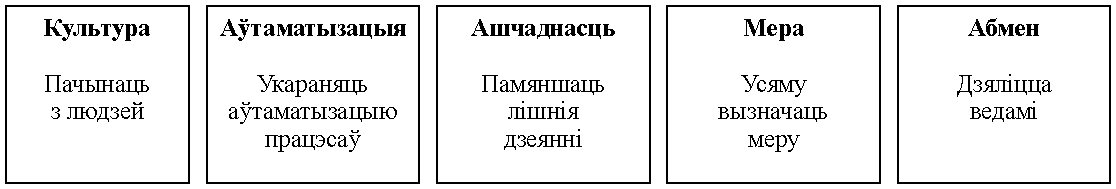
\includegraphics[width=\linewidth]{CALMS.pdf}
    \caption{мадэль CALMS}
    \label{fig:CALMS model}
\end{figure}

\vspace{-\baselineskip}
\subsubsection{Мадэль CALMS -- культура.}

Прыняцце метадалогіі DevOps пачалося з культуры.
У той час як матэрыяльная частка DevOps змяшчае новыя працэсы і
інструменты для бесперапыннай дастаўкі і інтэграцыі,
DevOps, усяго толькі, папулярнае слова,
калі "культура арганізацыі" не ахоплівае ўсе рэчы,
што ідуць у камплекце (Wilsenach 2015).

Галоўная ідэя DevOps -- змяніць культуру арганізацыі з
закрытых скрынь (асобныя ка\-ман\-ды) на адкрыты спосаб супрацоўніцтва
паміж імі.
Уцягнуць персанал тэхнічнай эксплуатацыі ў працэсы
распрацоўкі праграм. Акрамя таго, неабходна іх прысутнасць на
сходзе для планавання, агляду праектных каманд, каб яны маглі
падзяліцца ўласнымі ідэямі і ведамі ўжо на ранніх стадыях працэсу
распрацоўкі.
Humble і Molesky (2011 год) заўважылі, што абмен з ка\-ман\-дамі
тэхнічнай эксплуатацыі неабходны для распрацоўшчыкаў, і яны
павінны ў аднолькавай меры ўдзельнічаць у аналізе знаходжання
першапрычын ў выпадку вытворчых інцыдэнтаў.

Без разумення працэсаў, каторыя адбываюцца ўнутры іншых каманд
(тэхнічнай эксплуатацыі, тэсціравання), немагчыма дабіцца
палітыкі неабвінавачвання ў кампаніі.
Палітыка неабвінавачвання прадугледжвае прызнанне чалавечых памылак і
разглядае іх у якасці магчымасці палепшыць прадукцыйнасць кампаніі
пры дапамозе аналізу першапрычын і наступнага недапушчэння
аналагічных памылак.
Калі супрацоўнікі кампаніі не баяцца быць абвінавачанымі і
пакаранымі за памылкі, адкрываецца шлях да новых інавацый,
павялічваецца матывацыя і адданасць кампаніі.

У асяроддзі супрацоўніцтва знікае такая праблема, як перакладванне
адказнасці на іншыя каманды, дазваляе на ранніх стадыях знаходзіць
праблемы ў праграмных прадуктах або паслугах.

\subsubsection{Мадэль CALMS -- аўтаматызацыя.}
